\documentclass{article}

\usepackage[dblblindworkshop]{neurips_2026}

\usepackage[utf8]{inputenc}
\usepackage[T1]{fontenc}
\usepackage{graphicx}
\usepackage{hyperref}
\usepackage{url}
\usepackage{booktabs}
\usepackage{amsfonts}
\usepackage{nicefrac}
\usepackage{microtype}
\usepackage{xcolor}

\title{When Does Monitoring Long-Horizon Agents Lead to Better Performance?}
\workshoptitle{New In Machine Learning (NewInML)}

\author{Anonymous Author(s)}

\begin{document}

\maketitle

\begin{abstract}
Long-horizon language-model agents often rely on runtime monitors to detect degradation and trigger interventions in their workflows. We study whether such monitoring actually improves agent performance. Across behavioral sentinels, multiple models, and long-horizon tasks, we find that monitoring is not a free observation: there exists an ``observer effect'' where probes can alter the behavior of the agent they are meant to measure and that no single monitoring method dominates across all settings. More importantly, we find that the value of monitoring depends strongly on the exact recovery mechanism it triggers. Our results show that agent monitors should be evaluated jointly with the recovery systems they are paired with, rather than as standalone predictors.
\end{abstract}

\section{Introduction}

The use of agents like Claude Code and Codex has been drastically increasing for tasks that require maintaining goals and state over an extended period of time(i.e deep research, coding, etc).[CITATION] As these trajectories grow longer, however, agents can gradually lose important context and start hallucinating incorrect information[CITATION]. A natural response is to monitor an agent during execution and intervene whenever its behavior starts to degrade. This can include restarting the agent compacting its context or simply restructuring state before the agent continues execution[CITATION(S)].

The need to preserve agent behavior creates an appealing intuition: if we can detect degradation earlier and more accurately, we should be able to intervene at better times and improve task performance. This has drastic implications for all agent tasks, whether it be coding benchmarks like (...) or enterprise (\ldots{}.).

Much of agent monitoring can thus be viewed as a prediction problem: given an agent current behavior/state, determine whether it is likely to fail in the near future. Under this view, a more accurate monitor should naturally produce a better agent.

\textit{[insert a conditional prob math thing here explaining the above notion, or can put in experimental setup]}

We argue this view is incomplete; any runtime monitor is not necessarily a passive observer of an agent trajectory.

The most common form of monitoring introduces additional instructions or computations directly into the agent context[CITATION],  [maybe include a quick diagram example here as well]. We study one such class of monitors, which we call behavioral sentinels: canaries that an agent must maintain throughout a task and whose degradation can serve as a warning signal. For example, an agent might be asked to remember and update a small piece of state while simultaneously completing its primary task. The intuition here is if the agent fails to maintain the state before completing the underlying task, the sentinel can provide an early warning signal.

However, asking the agent to maintain such a signal can itself change the trajectory of an agent. Across our experiments, we find an observer effect: a probe cannot predict the degradation of an agent without playing some part in the degradation itself. Monitoring therefore is not always a free source of information, and higher quality signals do not automatically imply higher performance.

Detecting degradations is useful because the resulting signal eventually triggers an intervention. Intuitively, this means the value of a monitor may depend not just when it fires but what the system does afterwards. We study this interaction directly by evaluating monitoring under different recovery mechanisms. Specifically, to answer the question of whether the effect of monitoring depends on the recovery mechanism it is paired with, we compare recovery based on agent-generated context compaction with recovery that reconstructs state from an external source of truth.

Our experiments reveal that it does. Under lossy-agent generated compaction, carrying additional state can reduce the benefit of an otherwise well-timed intervention. However, when the state is reconstructed through deterministic regrounding, this penalty disappears and the monitoring setup can be beneficial.

Our work makes three primary contributions:
\begin{itemize}
  \item We characterize monitoring as an intervention rather than a free observation. Behavioral probes alter trajectories, producing an observer effect
  \item We experimentally isolate the interaction between monitoring and recovery. Holding the monitoring setup fixed, we show that changing how agent state is reconstructed can substantially change whether monitoring improves downstream performance.
  \item We evaluate monitoring as a complete systems problem. Across multiple models and long-horizon tasks, we find that no single monitoring strategy consistently dominates.
\end{itemize}

\section{Related Works}

\subsection{What has already been done}

Recent work has explored detecting degradation on agents before task completion

[Citation-> Doomed from the start] introduces the idea of utilizing probes over internal model activations to predict task failure and terminate struggling trajectories. [Citation] similarly detects agent drift from internal activation and uses activation steering to mitigate it during execution.

Other work has introduced explicit diagnostic probes: [Canary Tools], for example, inserts adversarially designed tools into an agent's context to expose weaknesses in tool-selection reasoning.

Together, these methods show us that agent failure can often be detected before task completion, whether it be internal representations, observing trajectories, or introducing probes

\textit{[Show diagram here of the three methods and agent]}

\subsection{What gap remains}

A newer line of work explores what should happen after degradation is detected. [Citation] combines early failure prediction with different restart strategies, showing us that preserving useful work across sessions can outperform a cold restart. [AgentRewind] further treats recovery as a state management problem, checkpointing both agent context and environment state, so execution can return to an earlier point after agent failure.

Separately work on long-horizon context management has shown that LLM-generated compaction is inherently lossy and can unpredictably discard important information that is needed for later sessions[CITATION].

\subsection{Why this paper is different}

Prior work therefore establishes two notions: agent failures can be monitored and that choosing the right recovery strategy matters. However, these components are typically evaluated separately. Monitoring work primarily asks whether a signal predicts a failure, while recovery work asks how best to restore or restart an agent once intervention occurs. To our knowledge, prior work has not studied how the monitoring mechanism itself interacts with agent state after intervention. We study this precise interaction explicitly. Using behavioral sentinels and passive monitors, we measure both signal quality and how observation changes task execution and recovery.

In particular, we hold the monitoring setup fixed while replacing lossy agent-generated compaction with deterministic external re-grounding, allowing us to precisely test whether the effect of monitoring changed depending on the recovery mechanism.

We need to ``get-to-the-point'' faster into our conclusions below

\section{Experiment Set up}

A little on experiment set up

\subsection{Agentic Tasks --- NO regard for observation methods}

incremental resets vs no resets --- how does performance differ?

incremental regrounding vs no regrounding --- how does performance differ?

\subsection{Error Recall --- JUST active observation}

Active probes vs baselines --- leads to pretty bad the precision / recall

This is because of ``observer effect'', where the extra chore confounds performance on the task itself

\subsection{Findings on when it's best to compact / re-retrieve context stored in agent state}

\section{Results}

\section{Discussion / Conclusion}

\clearpage
\section{Figures}

\begin{figure}[p]
  \centering
  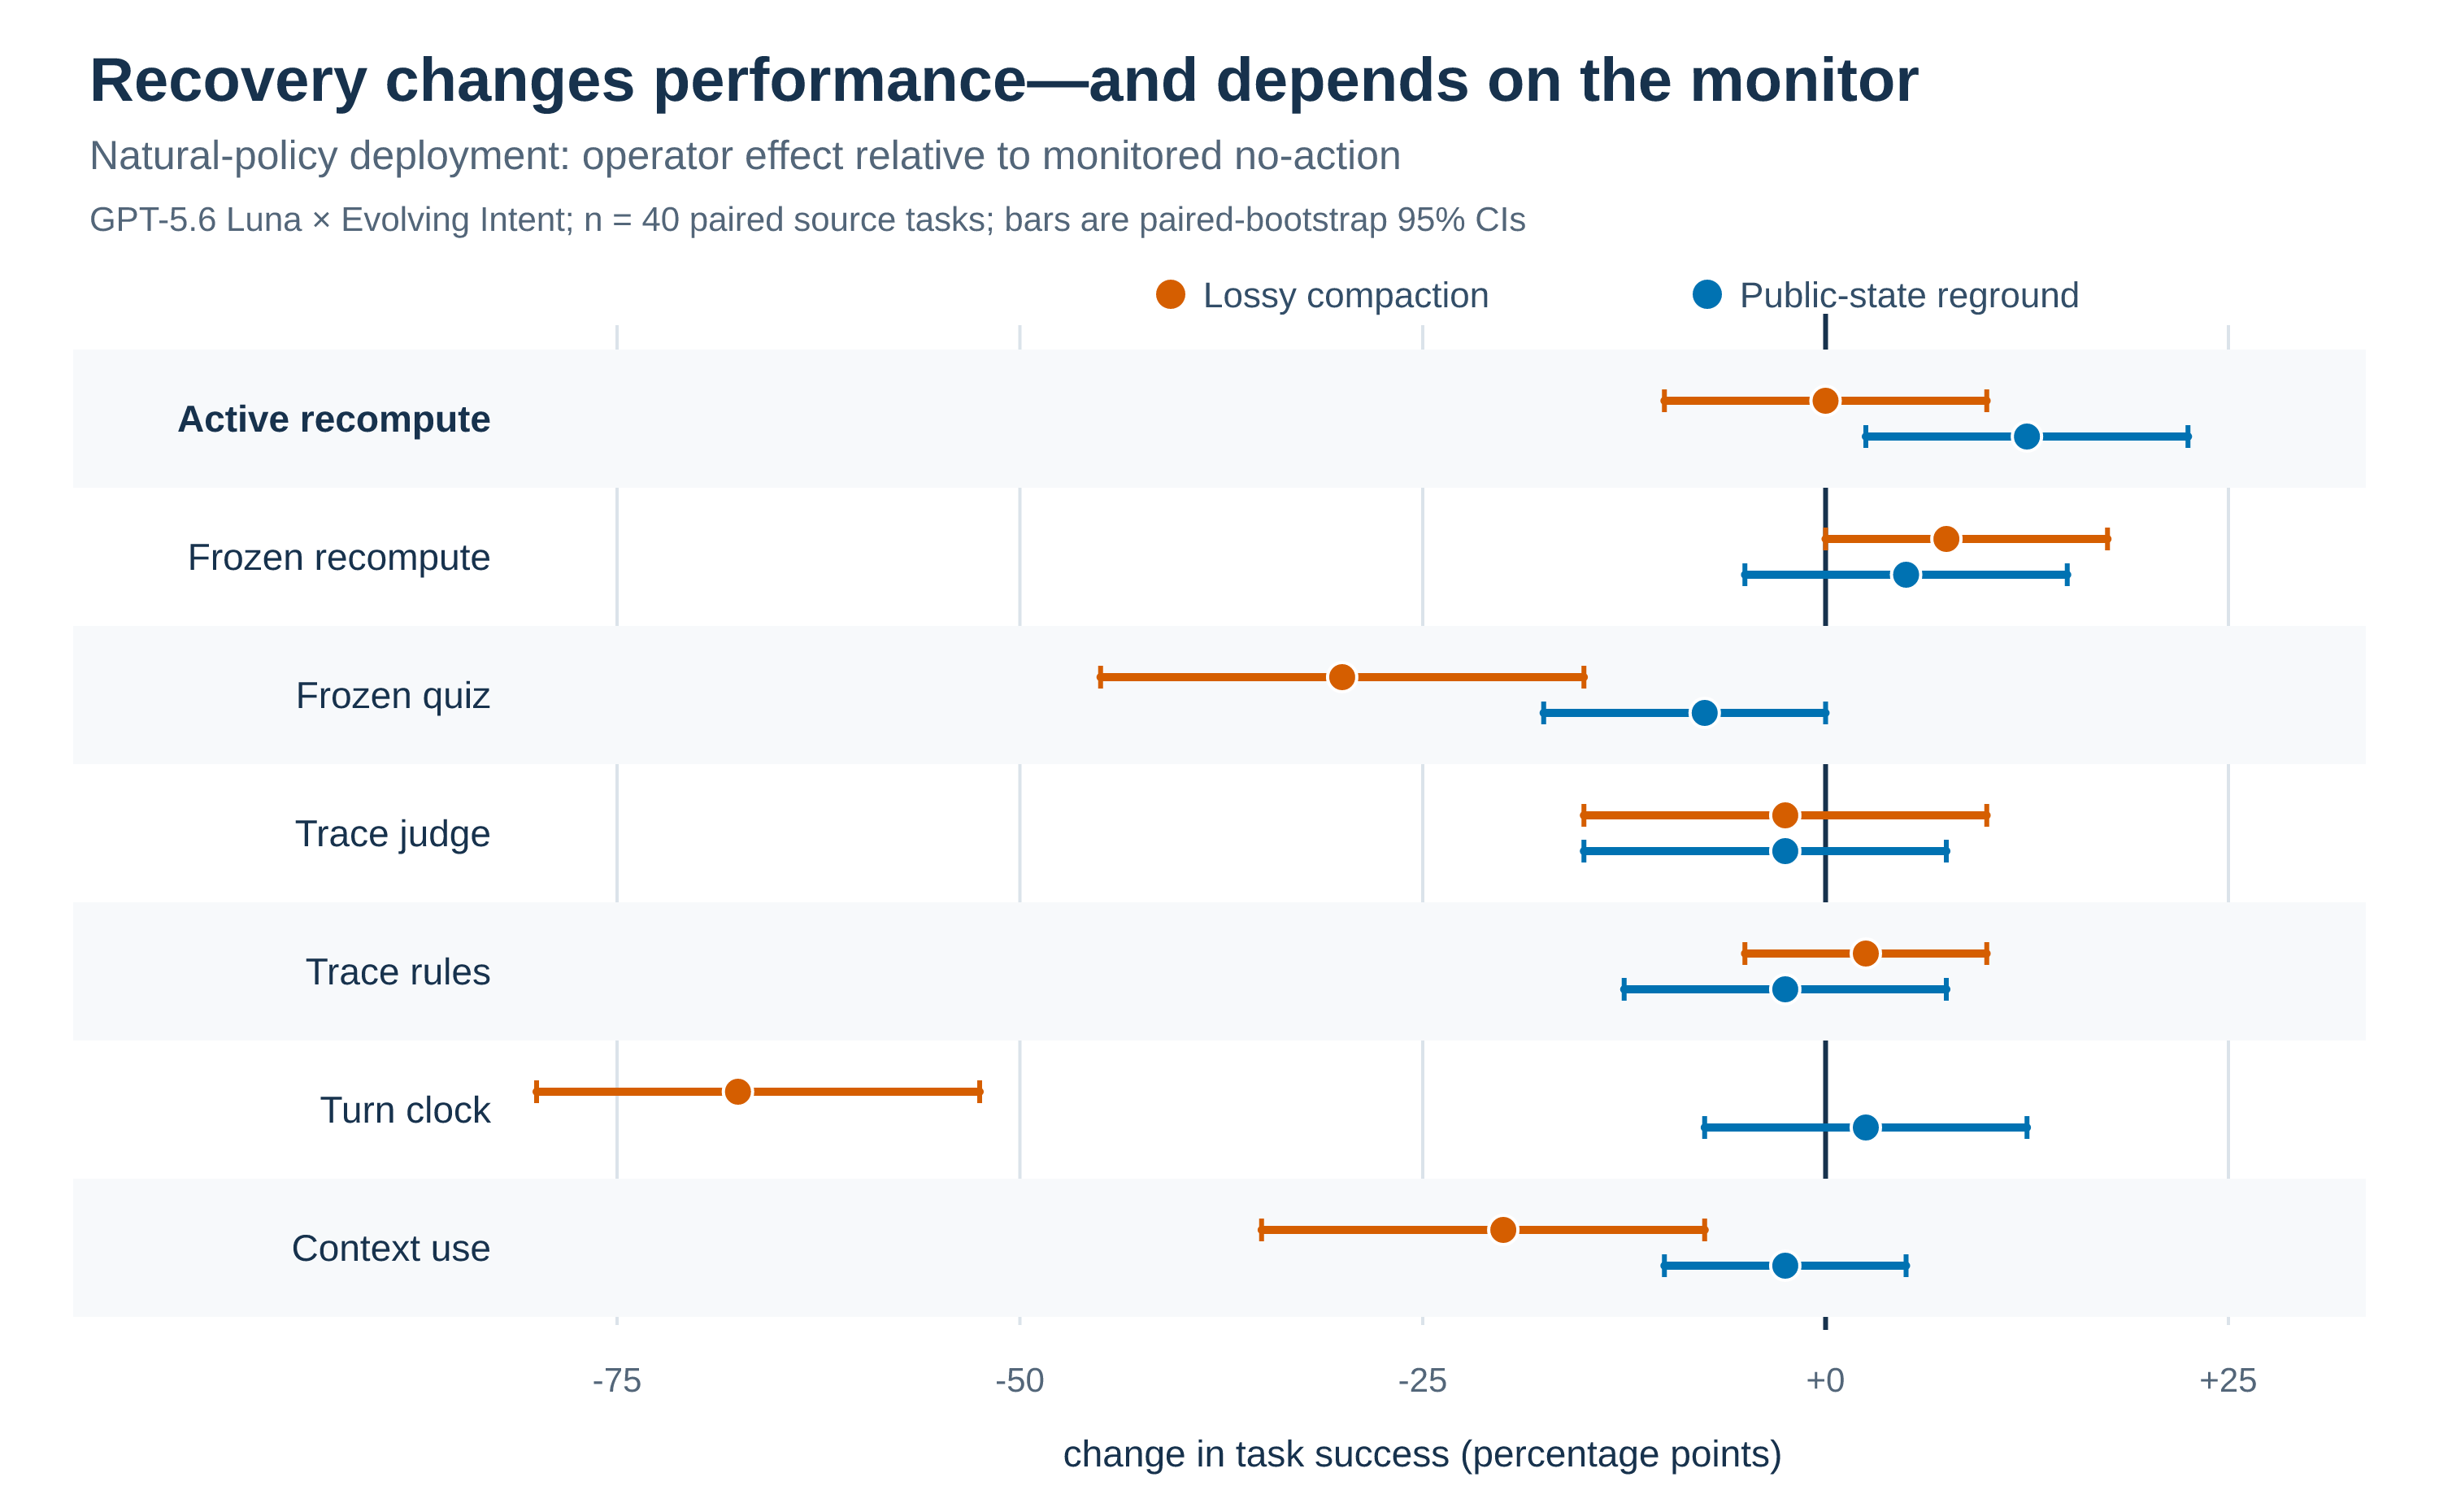
\includegraphics[width=\linewidth]{figures/01-recovery-operator-effects.png}
  \caption{Recovery-operator effects relative to monitored no-action in the natural-policy deployment. Lossy compaction and deterministic public-state regrounding produce different outcomes, and their effects vary with the paired monitoring method.}
  \label{fig:recovery-operators}
\end{figure}

\begin{figure}[p]
  \centering
  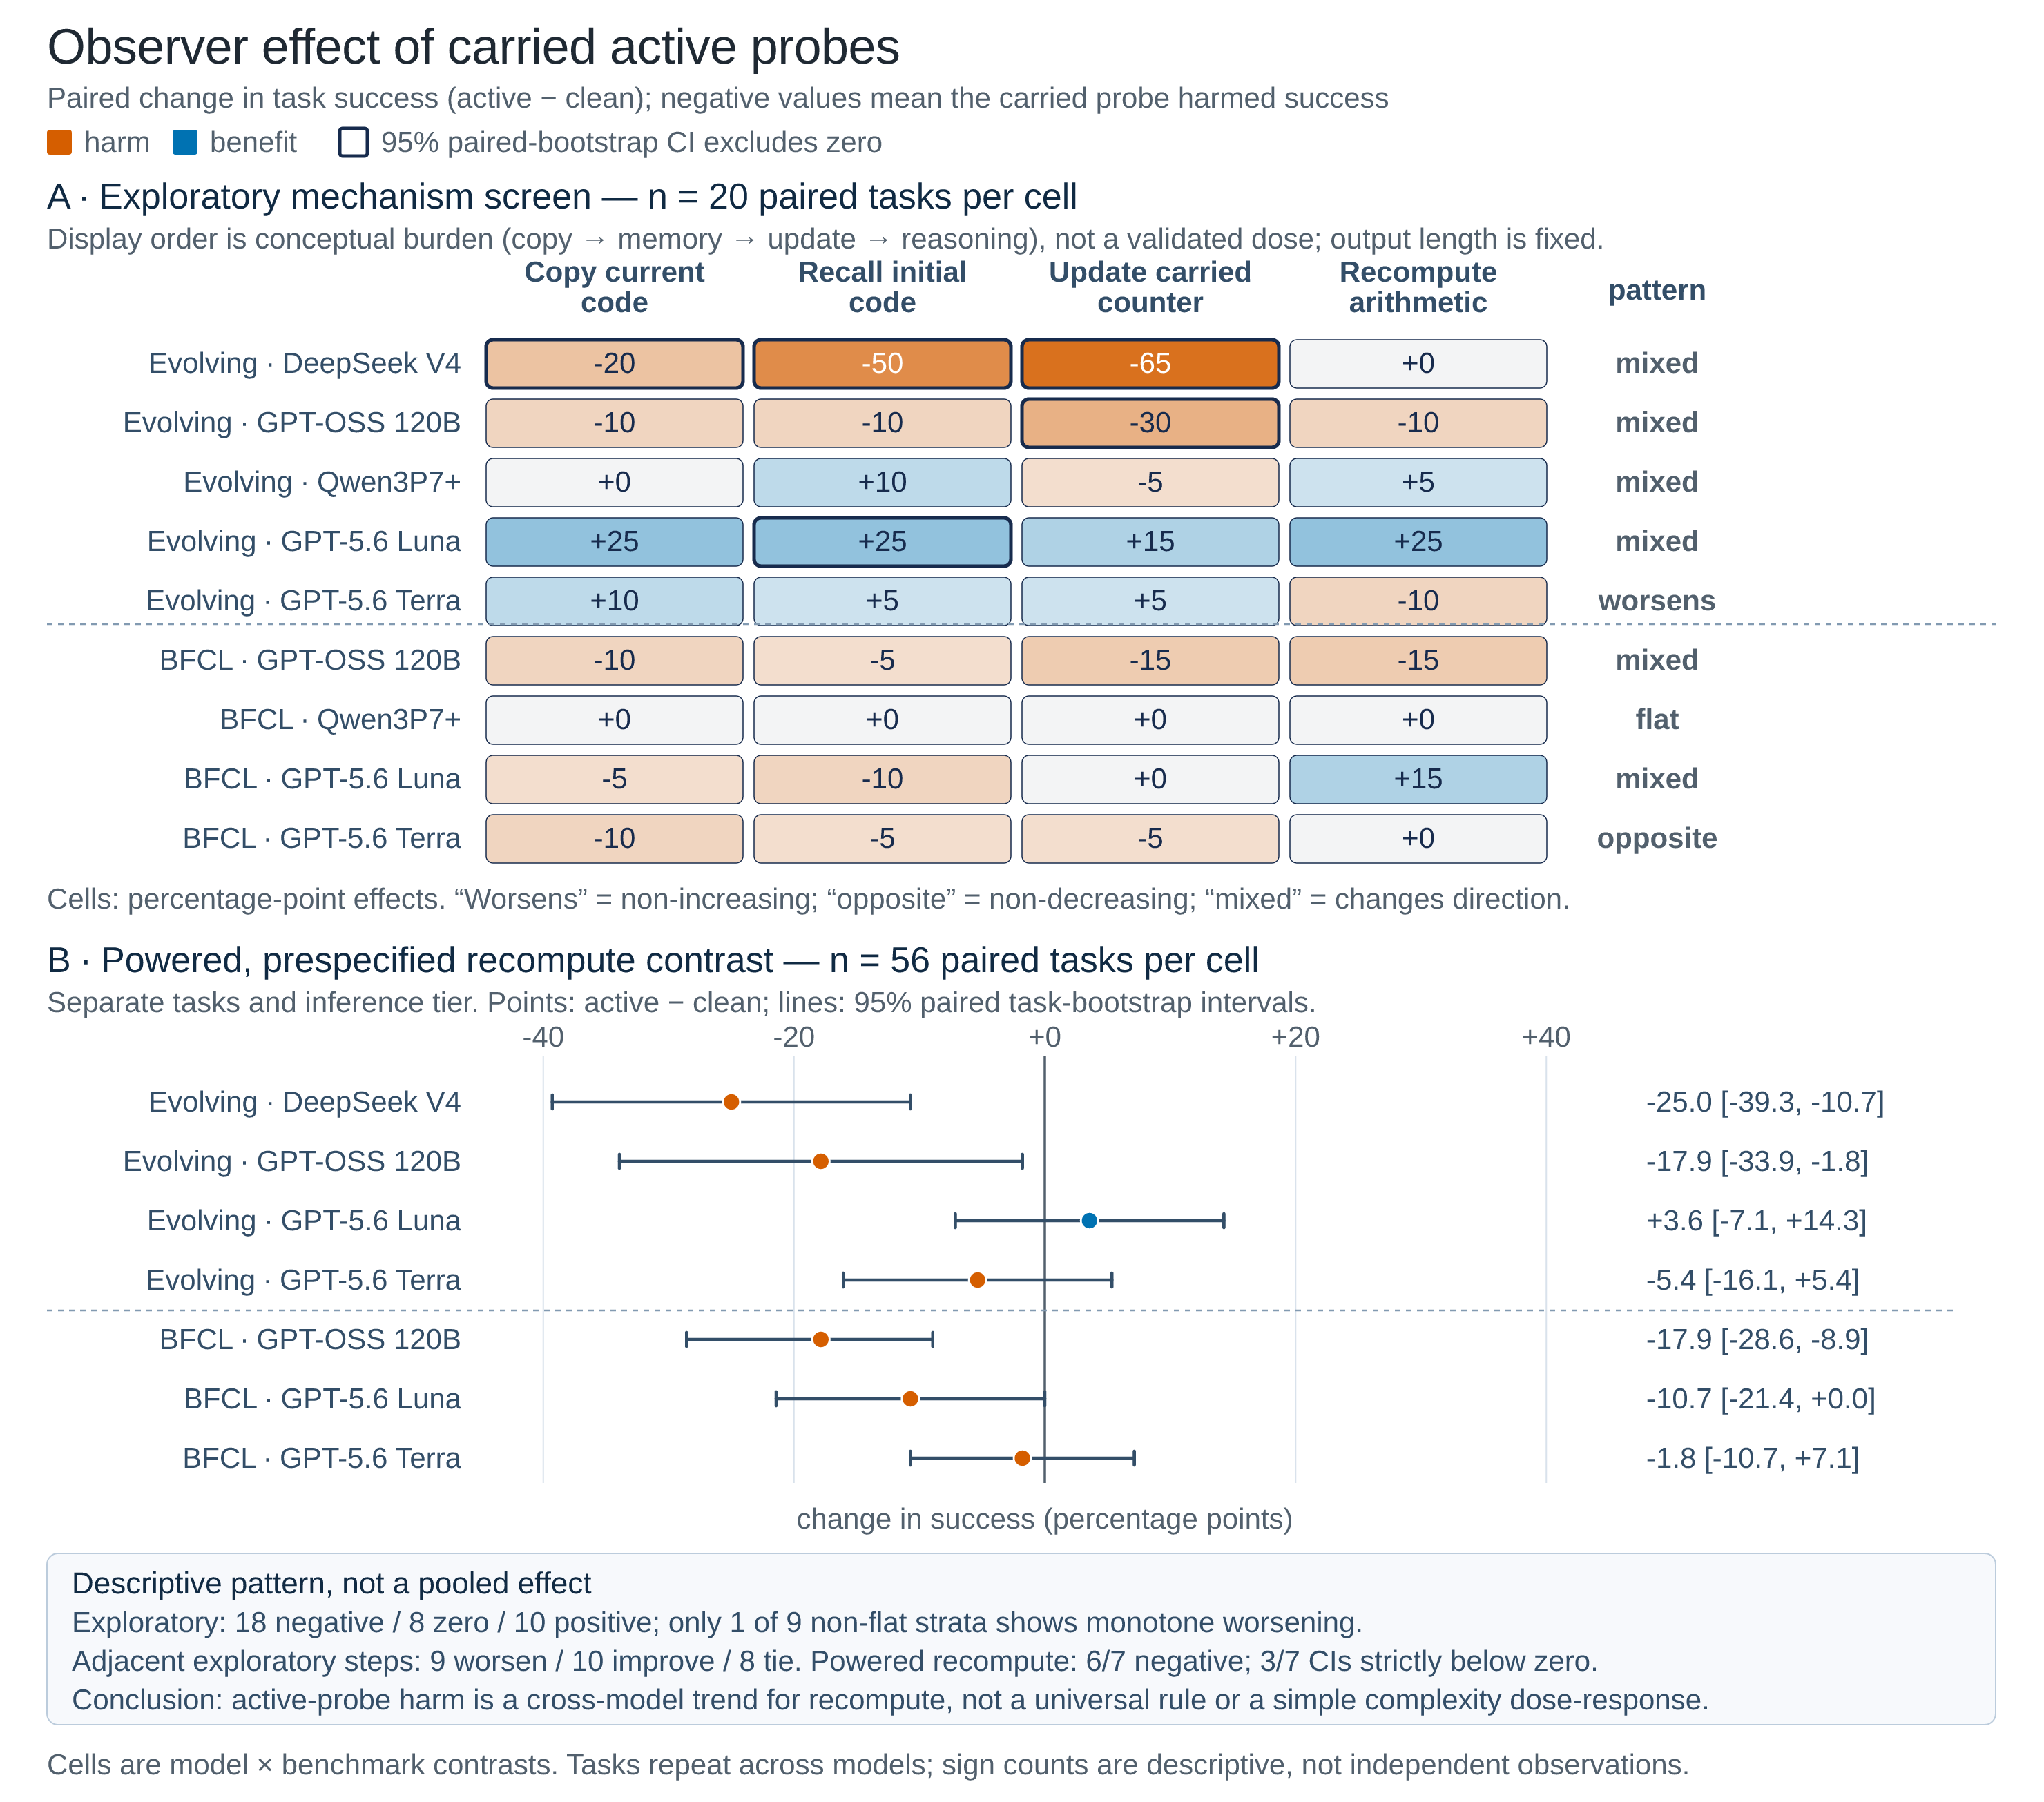
\includegraphics[width=\linewidth]{figures/02-active-probe-observer-effect.png}
  \caption{Observer effect of carried active probes. The lower panel is the powered, prespecified recomputation contrast; the upper mechanism screen is exploratory.}
  \label{fig:observer-effect}
\end{figure}

\begin{figure}[p]
  \centering
  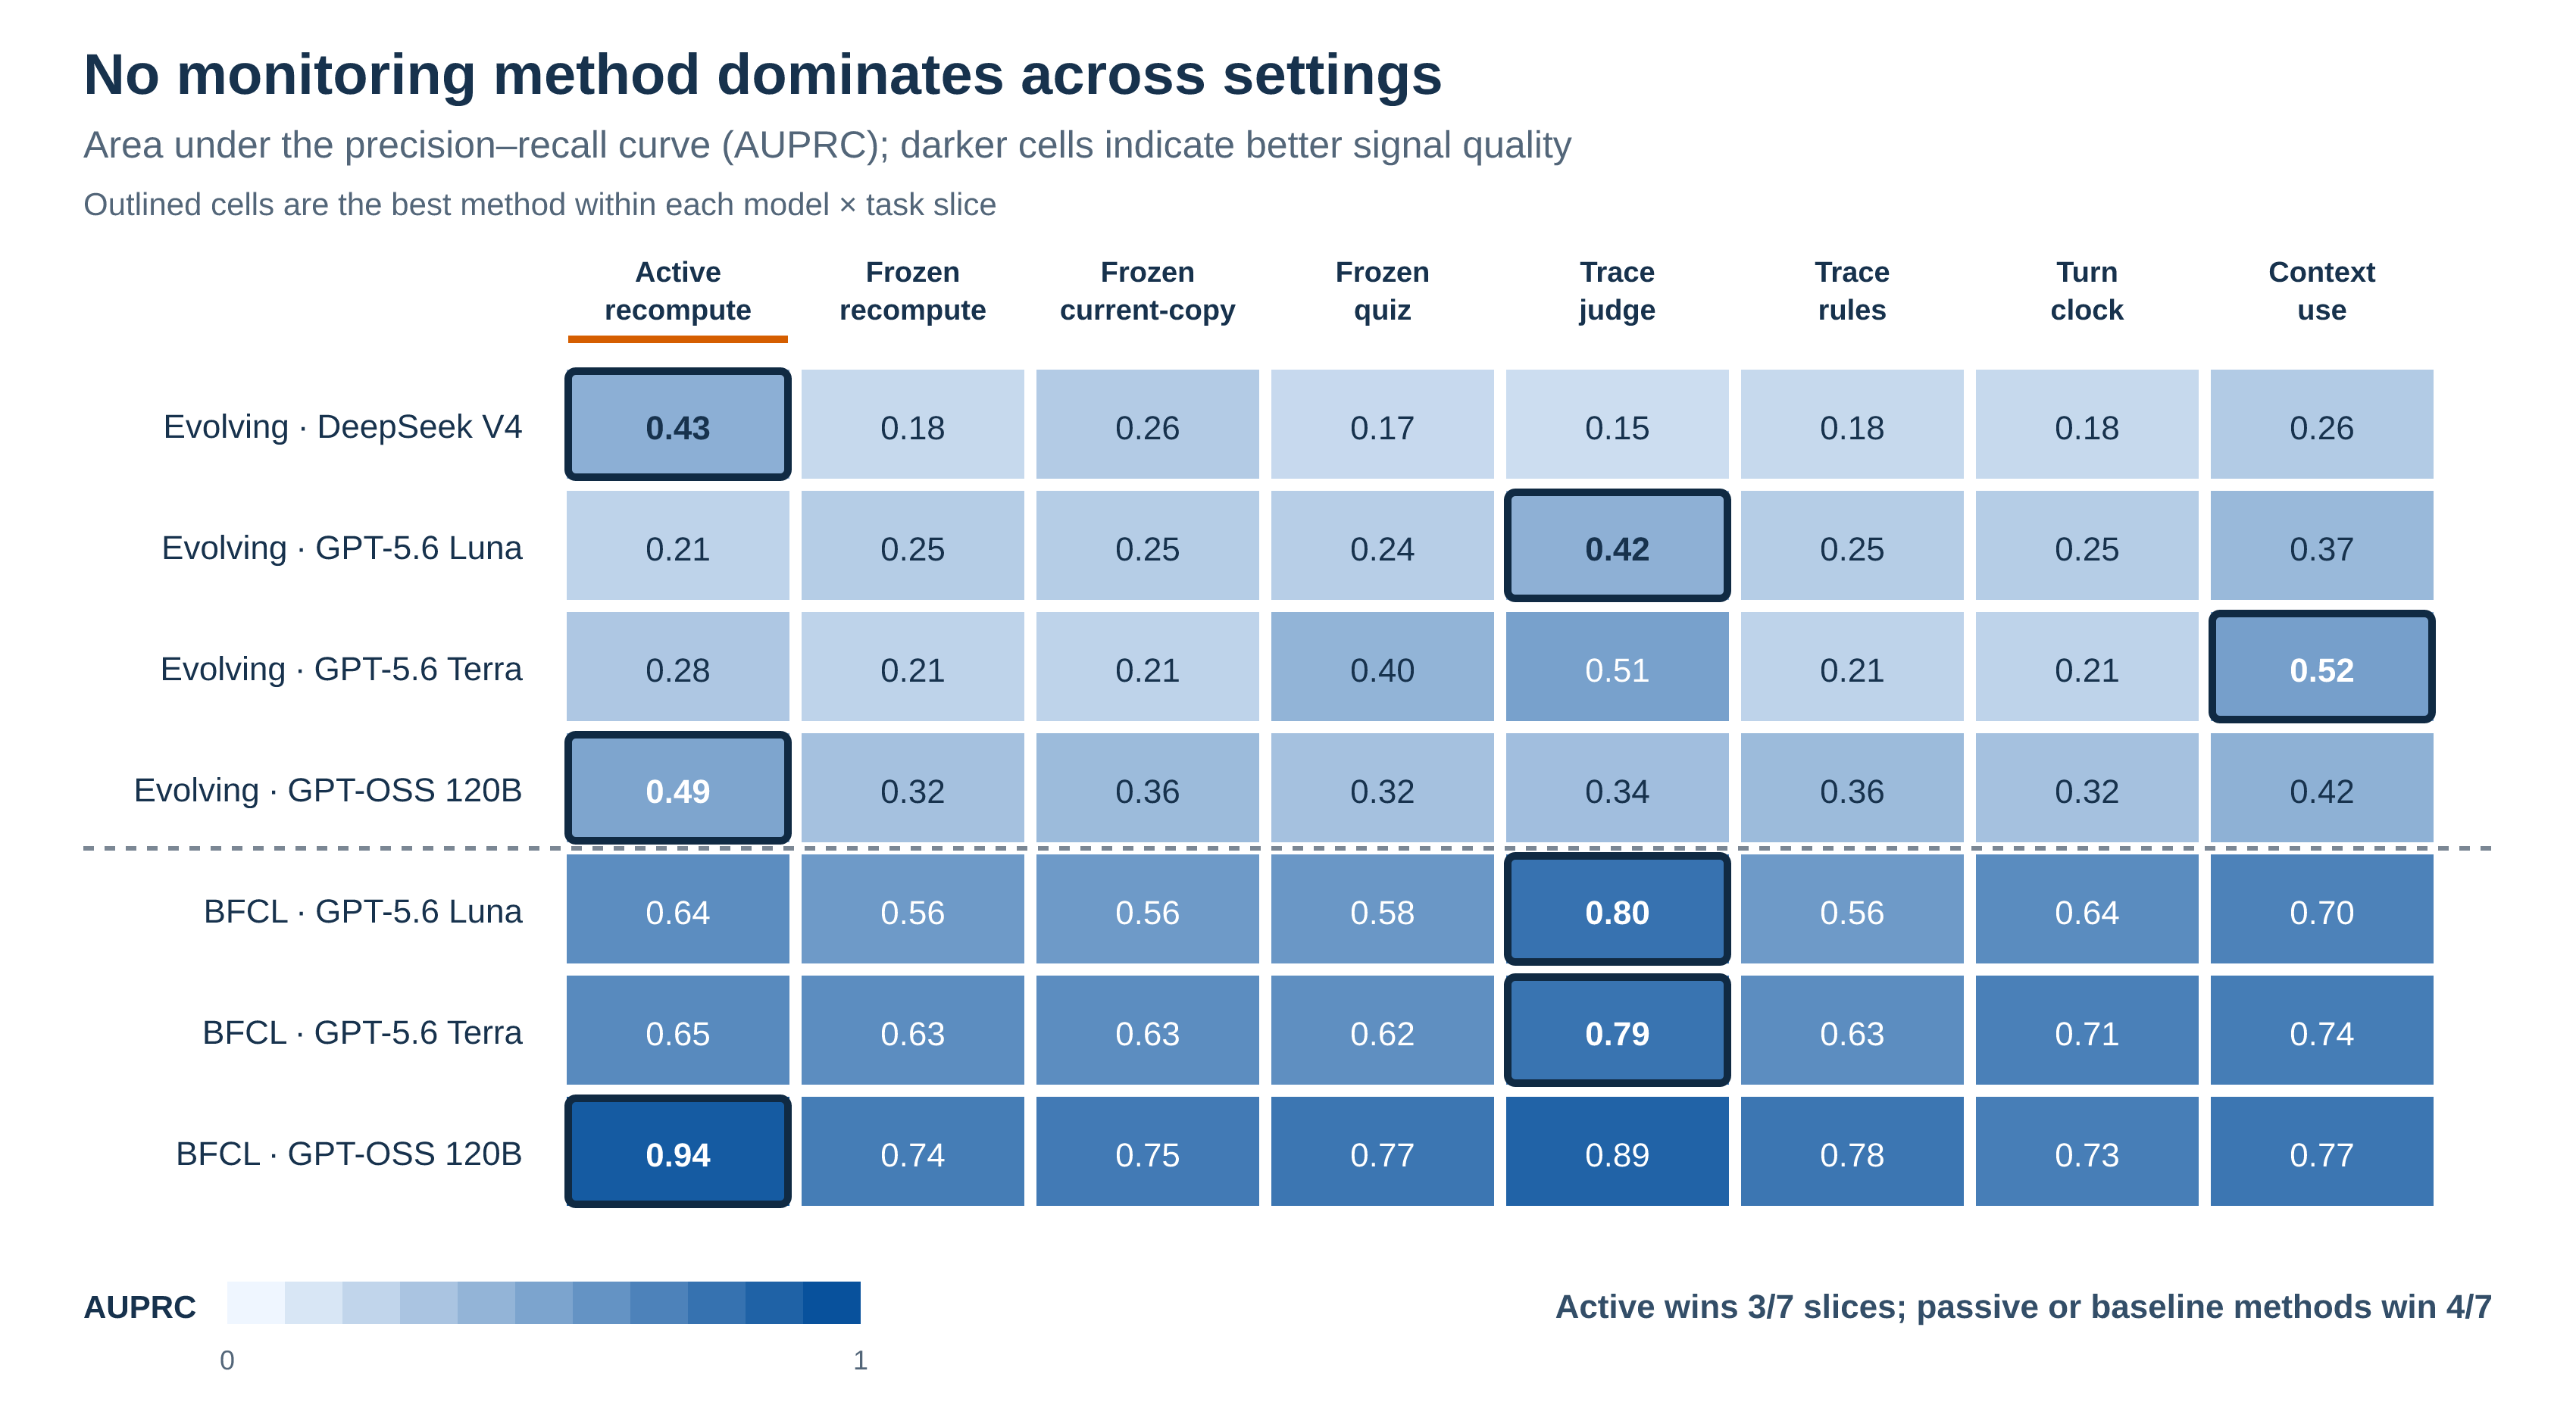
\includegraphics[width=\linewidth]{figures/03-signal-quality-auprc.png}
  \caption{Signal quality across every powered model-by-task slice. The identity of the best method varies across settings, so neither active, passive, nor baseline monitoring dominates universally.}
  \label{fig:signal-quality}
\end{figure}

\begin{figure}[p]
  \centering
  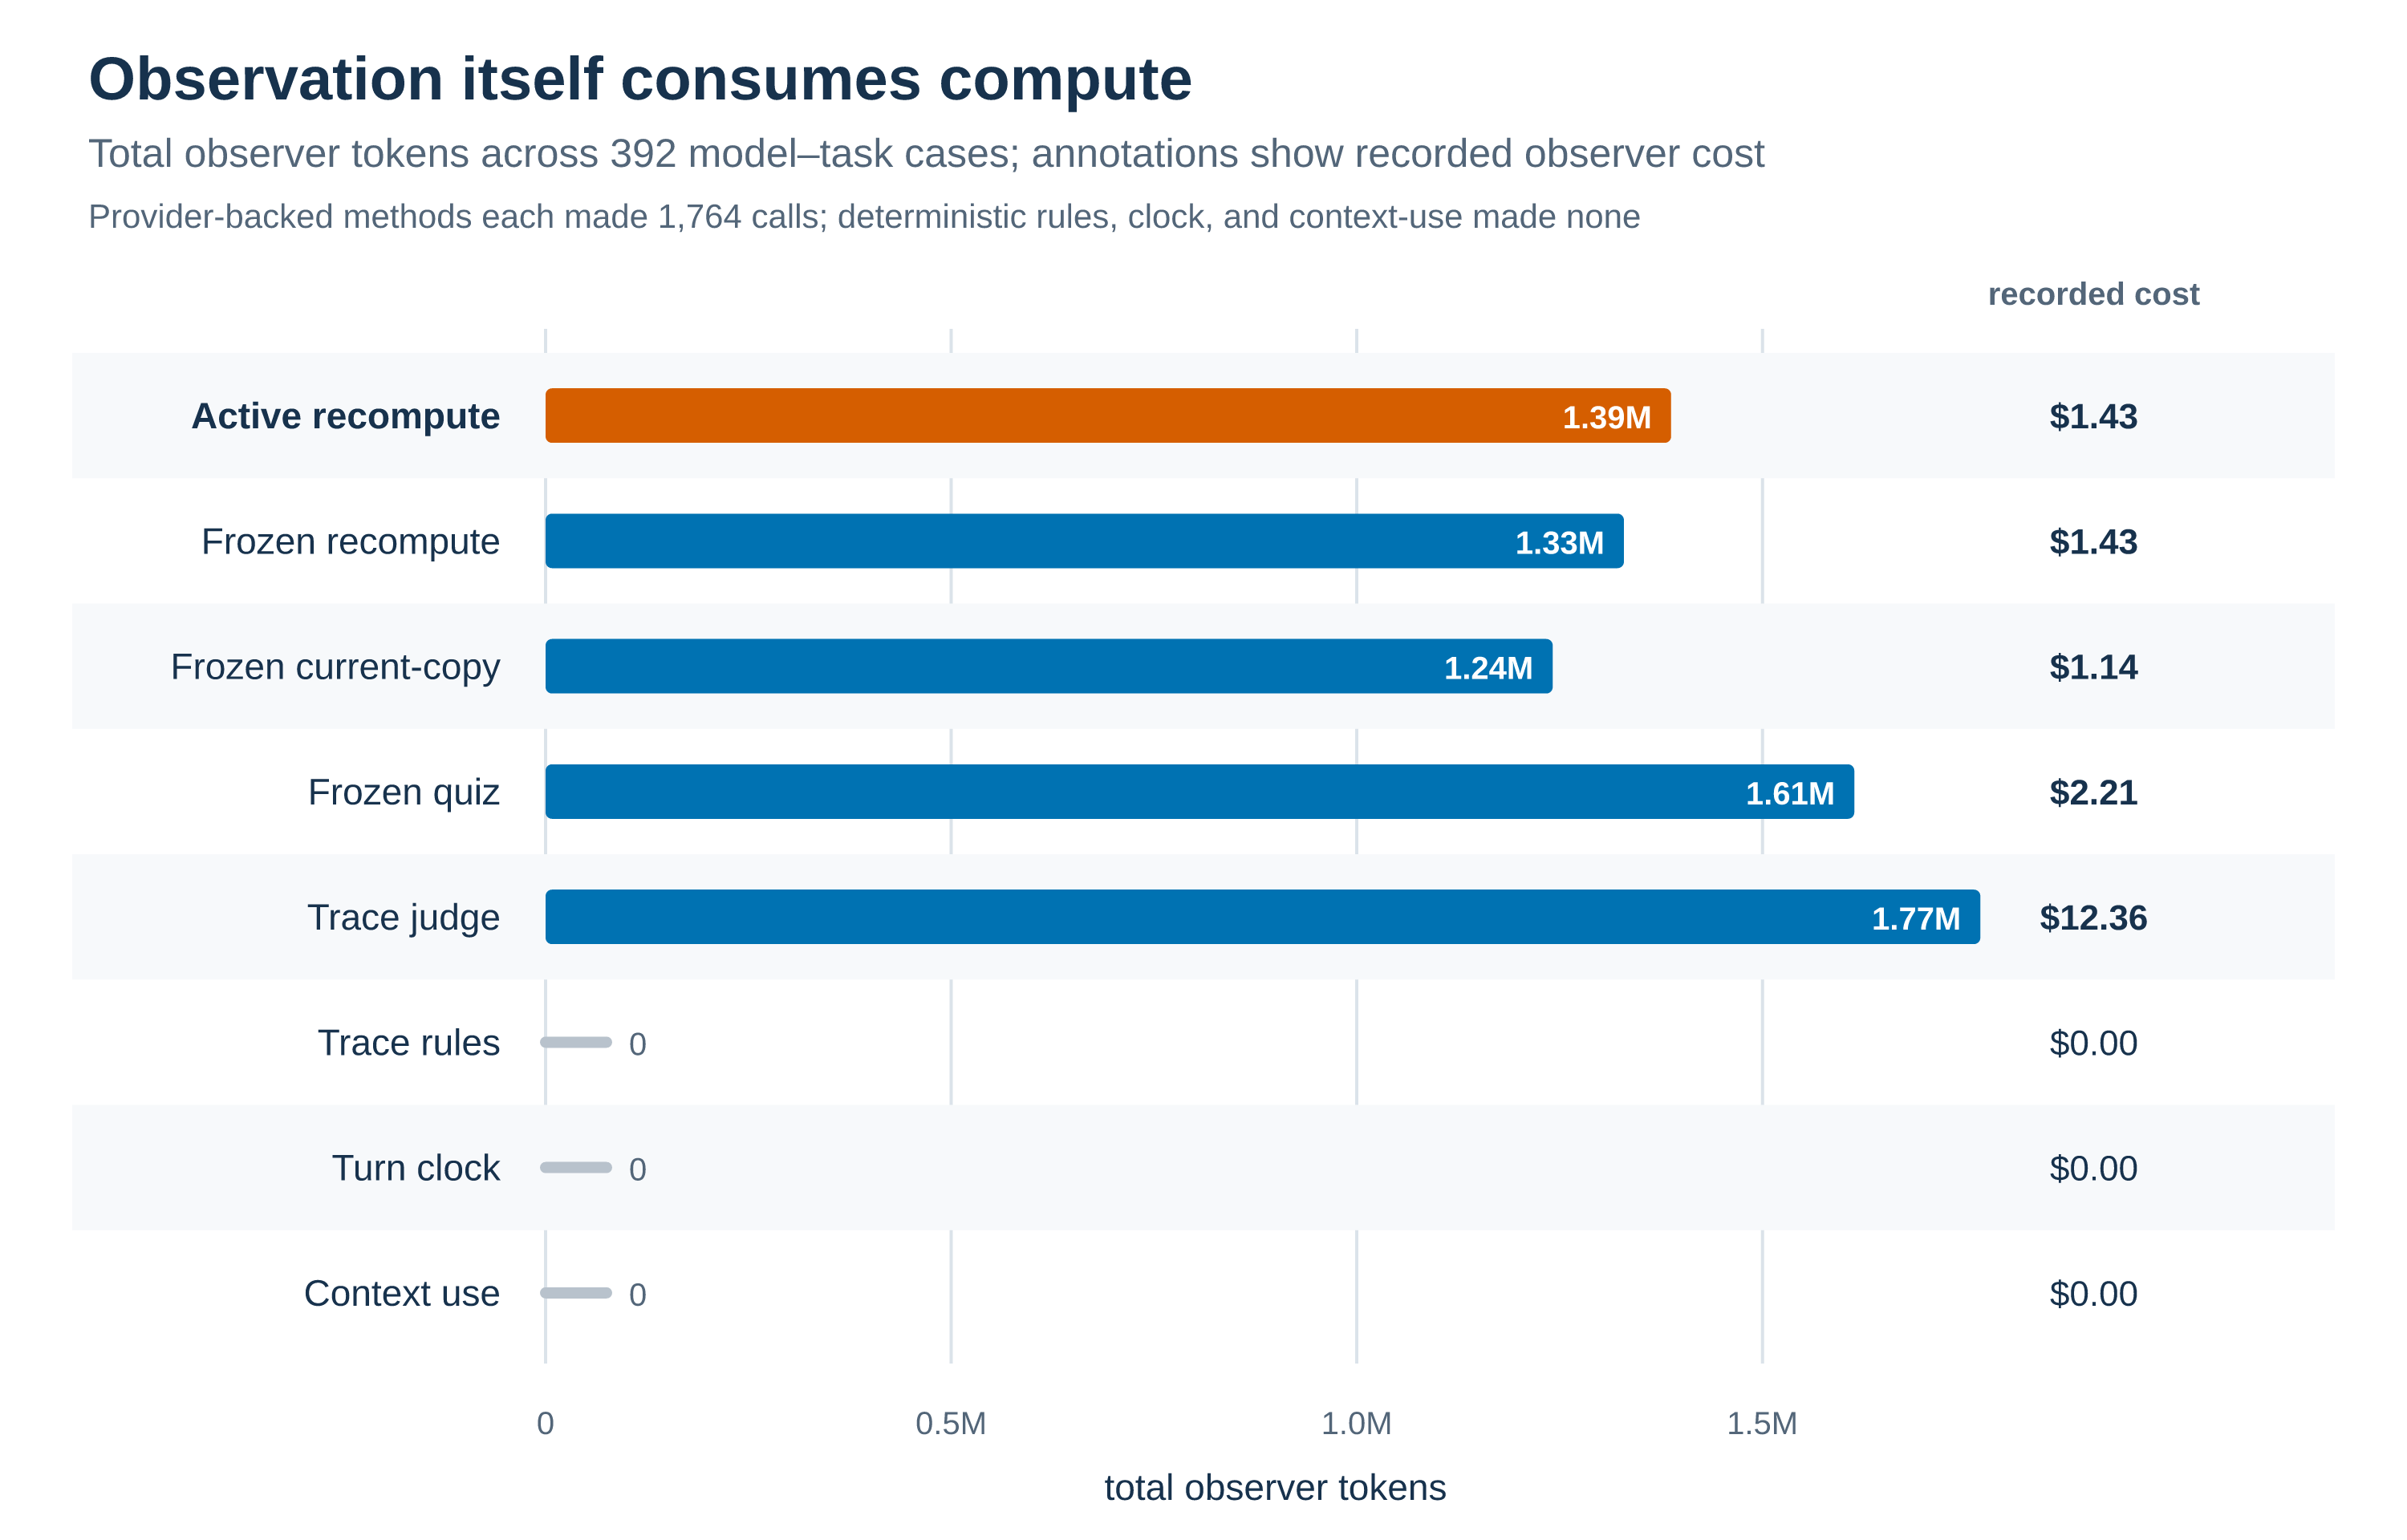
\includegraphics[width=\linewidth]{figures/04-observation-overhead.png}
  \caption{Compute used by observation itself. Provider-backed methods incur calls, tokens, and recorded cost; deterministic trace rules, clocks, and context-use add no provider calls.}
  \label{fig:observation-overhead}
\end{figure}

\clearpage
\section*{References}

\end{document}
